\documentclass{article}

\usepackage{amsmath}
\usepackage{graphicx}
\usepackage{wrapfig}
\usepackage[margin=.9in]{geometry}

\begin{document}
\title{Project 1 Design Doc}
\author{Stern Huang (sh972) \& Colin Huang (ch645)}
\maketitle
\section{Introduction}
This is a design document for the \textbf{Project 2: Fully Pipelined MIPS} of CS 3410 (Spring 2014). In it, we will be describing our mini processor is implemented. This document is intended for the instructors of CS 3410 to read and and better understand how our circuits work. \\

\section{Overview}
\begin{center}
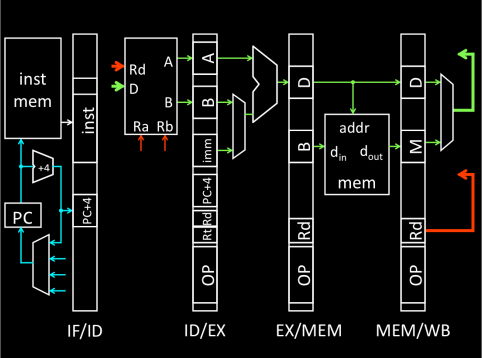
\includegraphics[scale=1.3]{pipeline.png} \\
Figure 1: Pipeline
\end{center}
\newpage
Creating the processor will consist of implementing 5 major pieces: \vspace{-3mm}\\ 
\begin{wrapfigure}{r}{0.35\textwidth}
\vspace{-1.7cm}
\begin{center}
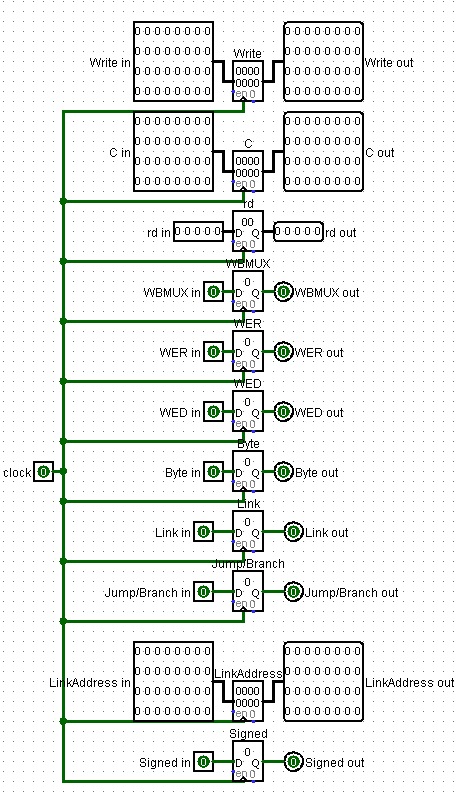
\includegraphics[scale=0.55]{isolator34.png} \\
Figure 2: Execute-Memory Isolator
\end{center}
\vspace{-1.5cm}
\end{wrapfigure}
\vspace{-0.7cm}
\begin{enumerate}
\item
\textbf{Pipeline Structure}: The implementation of a pipeline (Figure 1) requires the use of a clock as well as several registers to move data between different sections of the pipeline. We will refer to these as "\textbf{Isolators}" (Figure 2), as they isolate the various stages. Pipelining will be further explained in \textbf{Section 2.1}.

\item
\textbf{Decoding}: We must decode an instruction given by the Program ROM. This will tell the the register and the memory when to write, and the ALU what operation to perform. Various other bits will be outputted as well, which will be further explained in \textbf{Section 4}.

\item
\textbf{Execution}: The instructions that must be implemented are far more complicated than what a simple ALU is capable of. In order to carry out those instructions, we will create a larger Execute circuit, in which we use the ALU to perform specific operations. The Execute circuit will be further explained in \textbf{Section 5}.

\item
\textbf{Memory and Writeback}: After Execution, we will have to direct the computed value to where it needs to be used. This is usually the Memory or Writeback stage, but is also sometimes the Fetch stage. The Memory and Writeback implementation will be futher explained in \textbf{Section 6 and 7}.

\item
\textbf{Testing}: In order to test the functionality of our processor, we will write a program using the MIPS language and input it into the ROM. If the result is the expected result, we can conclude that our implementation of the processor is correct.
\end{enumerate}

\subsection{Circuit Diagram}
\begin{center}
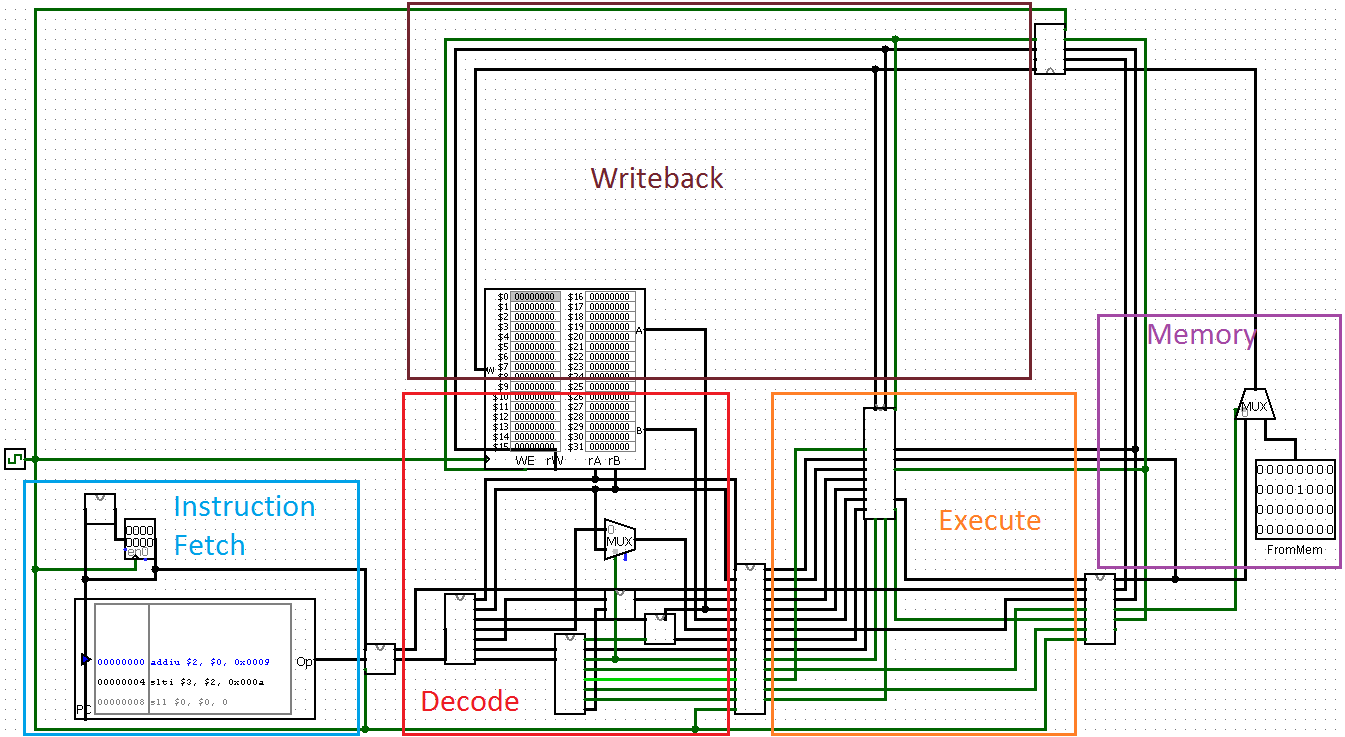
\includegraphics[scale=0.4]{Overview.png} \\
Figure 3: MIPS32 Circuit
\end{center}
The processor pipeline consists of 5 parts: \textbf{Instruction Fetch}, \textbf{Decode}, \textbf{Execute}, \textbf{Memory}, and \textbf{Writeback}. The clock on the far left determines when the data from one stage is transmitted to the next. This is done by the use of what we call \textbf{isolators}, which are simply a collections of registers that update on the rising edge of the clock. 

\section{The Fetch Stage}
The Fetch Stage is where the program instruction is extracted from the ROM. 
\subsection{Circuit Diagram}
\begin{wrapfigure}{r}{0.35\textwidth}
\vspace{-1.7cm}
\begin{center}
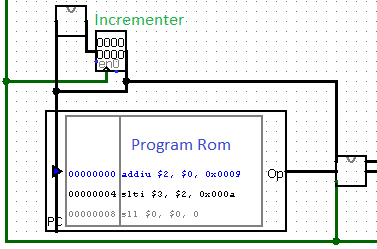
\includegraphics[scale=0.8]{Fetch.png} \\
Figure 4: Fetch
\end{center}
\vspace{-1.2cm}
\end{wrapfigure}
The Fetch stage has three main components: the \textbf{MIPS Program ROM},the \textbf{Incrementer} and the \textbf{Branching Circuit}. The MIPS Program ROM outputs 32-bit instruction codes depending on the inputted \textbf{program counter (PC)} to the isolator on the right. \\
The starting value of PC for any program is 0. Each subsequent instruction has PC 4 greater than that of the previous instruction. The incrementer will add 4 to the PC and store the result into the adjacent register on each clock tick. The register, however, is disabled when we must stall because of loading. \\
The branching circuit will usually output PC+4, as given by the incrementer. While branching, however, we it will instead output the jump or branch address. \\
The PC and the instruction code will be stored in the isolator to be used in the Decode stage. This is updated on each clock tick unless Load Stall is on, in which case the instruction code is halted within the isolator. 

\subsubsection{Submodule A: Incrementer}
\begin{wrapfigure}{r}{0.5\textwidth}
\vspace{-1.4cm}
\begin{center}
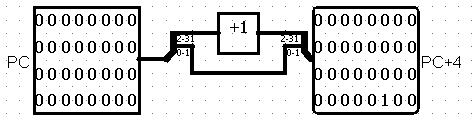
\includegraphics[width=0.5\textwidth]{Incrementer.png}\\
Figure 5: Incrementer
\end{center}
\vspace{-13mm}
\end{wrapfigure}
Figure 5 on the right is the Incrementer. We simply take the bits 2 through 32 and increase the value by 1. After appending back on the two least significant bits, we essentially have added 4 to the PC.

\subsubsection{Submodule B: Branch Circuit}
\begin{wrapfigure}{r}{0.45\textwidth}
\vspace{-1.5cm}
\begin{center}
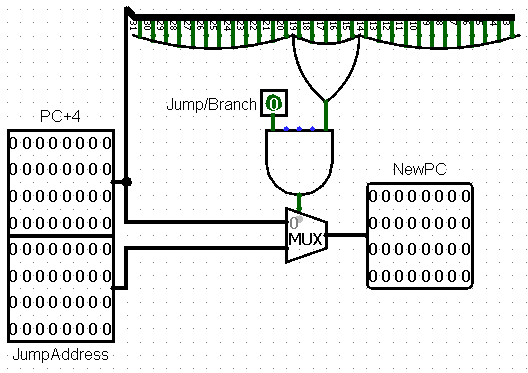
\includegraphics[width=0.42\textwidth]{FetchBranch.png} \\
Figure 6: Branching Circuit
\end{center}
\vspace{-1.9cm}
\end{wrapfigure}
Figure 6 is the branching circuit. It takes the inputs \textbf{PC+4}, \textbf{JumpAddress}, and \textbf{Jump/Branch}. The output PC is mainly determined by Jump/Branch. When we are not jumping or branching, we simply output PC+4. However, when we jump or branch, we select JumpAddress instead.

\subsection{Correctness Constraints}
The functional requirements for the circuit is as follows:
\begin{itemize}
\item
The \textbf{MIPS Program Rom} is correctly implemented, and has a valid program inputted. In other words, the ROM must take a 32 bit Program Counter input, and output a 32 bit instruction code. 

\item
The values Jump Address, Jump Enable, and Load Stall coming from the Memory stage must be correct. Load Stall is particularly important because if we were given a wrong value, the program could halt completely.
\end{itemize}
While not every MIPS instruction has been implemented, it will not change the functionality of the fetch stage. 

\subsection{Testing}
In order to verify the functional correctness of the incrementer and the Program ROM, we simply load a text file with MIPS instructions and turn on the clock. We expect the value of \textbf{PC} to increase by 4 every clock tick. We should also observe the instructions slowly scrolling through in the ROM. In order to test our Branching Circuit, we must write a program that involves branch and jump instructions.

\section{Instruction Decode}
Instruction Decode is where the 32 bit instruction code is read and decoded. Here we will figure out exactly the instruction is going to do, determining key values such as write enable and select bits of multiplexors to be used in later parts of the pipeline. 

\subsection{Circuit Diagram}
\begin{wrapfigure}{r}{0.42\textwidth}
\vspace{-1.5cm}
\begin{center}
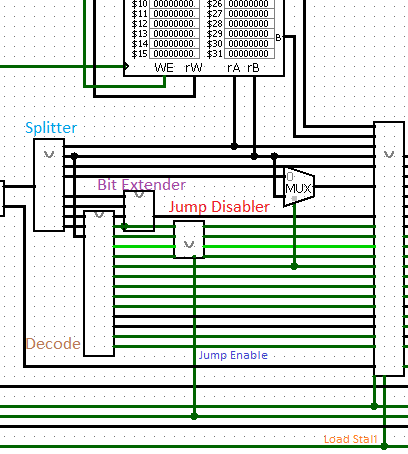
\includegraphics[width=.42\textwidth]{DecodeOut.png} \\
Figure 7: Decode
\end{center}
\vspace{-1.9cm}
\end{wrapfigure}
The decode circuit takes the PC and instruction code from the Fetch-Decode Isolator. The instruction code is then used to compute numerous values. 

The decode circuit consists of 6 components: 
\begin{enumerate}
\item
In the \textbf{splitter}, the instruction code is broken into more useful pieces.

\item
The \textbf{register} uses two of the register addresses from the splitter, reads out of those registers, and inputs them into the next isolator.

\item
The \textbf{decode} unit takes the first and last 6 bits of the instruction code and rt from the splitter and computes various values necessary for execution. Those values are then passed to the next isolator. 

\item
The \textbf{bit extender} extends the the immediate value for I and J type instructions into a 32 bit value. The method of extension is determined by the decode unit.
\end{enumerate}

\begin{enumerate}
\setcounter{enumi}{4}
\item
The \textbf{jump disabler} stops an instruction from doing anything. This is necessary to cancel out an instruction that is already fed into the pipeline when we want to jump or branch.

\item
The MUX will determine which register we will write back to. In R-type instructions, the write-back register address is located in bits 11 to 15. However, in I type instructions, the write-back register address is located in bits 16-20. This MUX will choose between the two.
\end{enumerate}

\subsubsection{Submodule A: Splitter}
\begin{wrapfigure}{r}{0.4\textwidth}
\vspace{-1.3cm}
\begin{center}
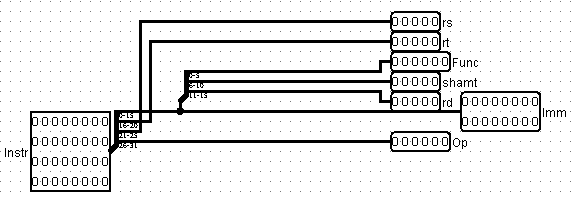
\includegraphics[scale=0.6]{Split.png} \\
Figure 8: Split
\end{center}
\end{wrapfigure}
Here, we can see the splitter break up the instruction code into several more useful pieces. Bits 0 to 15 make up the \textbf{immediate code}, which will be used in I type instructions. These 16 bits are then split into \textbf{function code}, \textbf{shift amount}, and \textbf{rd} which will be used in R type instructions. We will also have \textbf{Op} (bits 26 to 31) to determine the operation, and \textbf{rt} (bits 16 to 20) and \textbf{rs} (bits 21 to 25), the register addresses to be used.

\subsubsection{Submodule B: Decode}
The following table shows the desired outputs of each instruction:
\small
\begin{center}
\begin{tabular}{|c|c|c|c|c|c|c|c|c|} \hline
& \textbf{ALU} & \textbf{MUX 1} & \textbf{MUX 2} & \textbf{Write} & \textbf{Write} & \textbf{Shift} && \\
\textbf{Instruction} & \textbf{code} & \textbf{(Execute)} & \textbf{(Writeback)} & \textbf{Enable 1} & \textbf{Enable 2} & \textbf{Selector} & \textbf{Signed} & \textbf{Extend}\\ \hline
ADDIU & 001x & 1 & 0 & 1 & 0 &&&10\\ \hline
ANDI & 1000 & 1 & 0 & 1 & 0 &&&00\\ \hline
ORI & 1010 & 1 & 0 & 1 & 0 &&&00\\ \hline
XORI & 1100 & 1 & 0 & 1 & 0 &&&00\\ \hline
SLTI & 1111 & 1 & 0 & 1 & 0 &&1&10\\ \hline
SLTIU & 1111 & 1 & 0 & 1 & 0 &&0&10\\ \hline
ADDU & 001x & 0 & 0 & 1 & 0 &&&\\ \hline
SUBU & 011x & 0 & 0 & 1 & 0 &&&\\ \hline
AND & 1000 & 0 & 0 & 1 & 0 &&&\\ \hline 
OR & 1010 & 0 & 0 & 1 & 0 &&&\\ \hline
XOR & 1100 & 0 & 0 & 1 & 0 &&&\\ \hline
NOR & 1110 & 0 & 0 & 1 & 0 &&&\\ \hline
SLT & 1111 & 0 & 0 & 1 & 0 &&1&\\ \hline
SLTU & 1111 & 0 & 0 & 1 & 0 &&0&\\ \hline
MOVN & 1011 & 0 & 0 & 1 & 0 &&&\\ \hline
MOVZ & 1001 & 0 & 0 & 1 & 0 &&&\\ \hline
SLL & 000x & 0 & 0 & 1 & 0 & 0&&\\ \hline
SRL & 0100 & 0 & 0 & 1 & 0 & 0&&\\ \hline
SRA & 0101 & 0 & 0 & 1 & 0 & 0&&\\ \hline
SLLV & 000x & 0 & 0 & 1 & 0 & 1&&\\ \hline
SRLV & 0100 & 0 & 0 & 1 & 0 & 1&&\\ \hline
SRAV & 0101 & 0 & 0 & 1 & 0 & 1&&\\ \hline
LUI & 001x & 1 & 0 & 1 & 0 &&&01\\ \hline
J & xxxx & 1 & 0 & 0 & 0 &&&x1 \\ \hline
JR & xxxx & 0 & 0 & 0 & 0 &&& \\ \hline
JAL & xxxx & 1 & 0 & 1 & 0 &&&x1 \\ \hline
JALR & xxxx & 0 & 0 & 1 & 0 &&& \\ \hline
BEQ & 001x & 1 & 0 & 0 & 0 &&&10 \\ \hline
BNE & 001x & 1 & 0 & 0 & 0 &&&10 \\ \hline
BLEZ& 001x & 1 & 0 & 0 & 0 &&&10 \\ \hline
BGTZ& 001x & 1 & 0 & 0 & 0 &&&10 \\ \hline
BLTZ& 001x & 1 & 0 & 0 & 0 &&&10 \\ \hline
BGEZ& 001x & 1 & 0 & 0 & 0 &&&10 \\ \hline
LW & 001X & 1 & 1 & 0 & 1 &&0& 10 \\ \hline
LB & 001X & 1 & 1 & 0 & 1 &&1& 10 \\ \hline
LBU & 001X & 1 & 0 & 0 & 0 &&0& 10 \\ \hline
SW & 001X & 1 & 0 & 0 & 0 &&0& 10 \\ \hline
SB & 001X & 1 & 0 & 0 & 0 &&0& 10 \\ \hline
\end{tabular} \vspace{2mm}\\
For the following table, the values for instructions of Project 1 are all set to 0.
\begin{tabular}{|c|c|c|c|c|c|c|} \hline
& \textbf{Load/Store} & \textbf{Jump/Branch} && \textbf{Comp} & & \\ 
\textbf{Instruction} & \textbf{Byte} & \textbf{Enable} & \textbf{Link} & \textbf{Code} & \textbf{Branch} & \textbf{R Jump} \\ \hline
J &0& 1 & 0 & 000 & 0 & 0 \\ \hline
JR &0& 1 & 0 & 000 & 0 & 1 \\ \hline
JAL &0& 1 & 1 & 000 & 0 & 0 \\ \hline
JALR &0& 1 & 1 & 000 & 0 & 1 \\ \hline
BEQ &0& 1 & 0 & 010 & 1 & 0 \\ \hline
BNE &0& 1 & 0 & 011 & 1 & 0 \\ \hline
BLEZ &0& 1 & 0 & 100 & 1 & 0 \\ \hline
BGTZ &0& 1 & 0 & 111 & 1 & 0 \\ \hline
BLTZ &0& 1 & 0 & 101 & 1 & 0 \\ \hline
BGEZ &0& 1 & 0 & 110 & 1 & 0 \\ \hline
LW & 0 & 0 & 0  &000& 0&0 \\ \hline
LB & 1 & 0 & 0  &000& 0&0 \\ \hline
LBU & 1 & 0 & 0  &000& 0&0 \\ \hline
SW & 0 & 0 & 0  &000& 0&0 \\ \hline
SB & 1 & 0 & 0 &000& 0&0 \\ \hline
\end{tabular}
\end{center}
\normalsize
Any x's or missing fields mean that there is no preference between 0's and 1's. Notable variables include:
\begin{enumerate}
\item
\textbf{MUX 1}: This MUX select bit determines whether or not we are using an immediate value within Execute.

\item
\textbf{MUX 2}: This MUX select bit determines whether we are writing to the register from the ALU or from Memory.

\item
\textbf{Write Enable 1}: This determines whether or not we are writing to the register.

\item
\textbf{Write Enable 2}: This determines whether or not we are writing to Memory.

\item
\textbf{Shift Selector}: This bit determines whether the shift amount is from a register or from the 32 bit instruction code. (1 for register, 0 for instruction code)

\item
\textbf{Signed}: This bit determines whether the Less Than comparison considers the integers as signed or unsigned. (1 for signed, 0 for unsigned)

\item
\textbf{Extend}: This two bit code determines how the immediate value will be extended. Bit 1 determines whether we or sign extending or zero extending on the left. Then, bit 0 determines whether or not we must shifting the extended \textit{immediate} by 16 digits. Bit 0 also specifies when we are extending a 26 bit instruction index for Jumps.

\item
\textbf{Load/Store Byte}: This bit differentiates Load and Store word instructions from their Byte counterparts.

\item
\textbf{Jump/Branch Enable}: This bit is on when the instruction involves jumping to another program counter.

\item
\textbf{Link}: This bit specifies whether a Jump is linking. 

\item
\textbf{Comp Code}: This 3 bit code specifies the operation when we determine whether to take a branch or not.

\item
\textbf{Branch}: This bit specifies whether a jumping instruction is branching.

\item
\textbf{R Jump}: This bit specifies whether or not our jump address is coming from a register or the immediate output. 

\end{enumerate}

\noindent Figure 9 shows the Decode subcircuit. Decoding is done in two major parts: \vspace{-1cm}\\
\begin{wrapfigure}{r}{0.6\textwidth}
\vspace{-.1cm}
\begin{center}
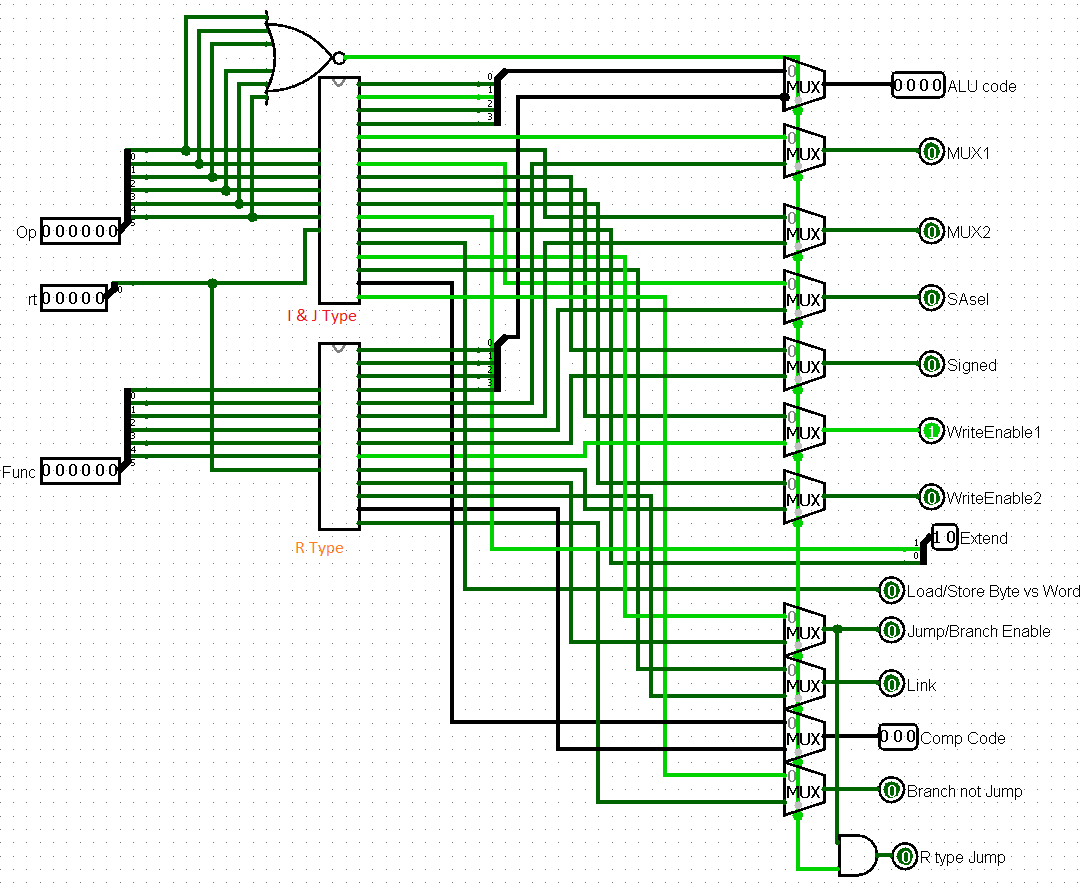
\includegraphics[width=0.63\textwidth]{Decoder.png} \\
Figure 9: Decode (subcircuit)
\end{center}
\vspace{-2cm}
\end{wrapfigure}
\begin{enumerate}
\item
For \textbf{I and J type instructions}, the operation is decided by \textbf{opcode} (bits 26 to 31) and \textbf{rt} (bits 16 to 20). Combinational analysis is then used on these 6 bits to determine output values.

\item
For \textbf{R type instructions}, \textbf{opcode} will be 000000, and the operation will be determined \textbf{function code} (bits 0 to 5) and \textbf{rt} (bits 16 to 20). Once again, we use combinational analysis to determine outputs.
\end{enumerate}
The XNOR gate in the circuit determines whether the instruction is R type or I/J type. The resulting bit is then used as the select bit for the multiplexors at the end. Because R type instructions have no immediate value, we simply output the value for \textbf{Extend} from the I and J type combinational analysis circuit.

\newpage

\subsubsection{Submodule C: Bit Extender}

\begin{wrapfigure}{r}{.6\textwidth}
\vspace{-1.4cm}
\begin{center}
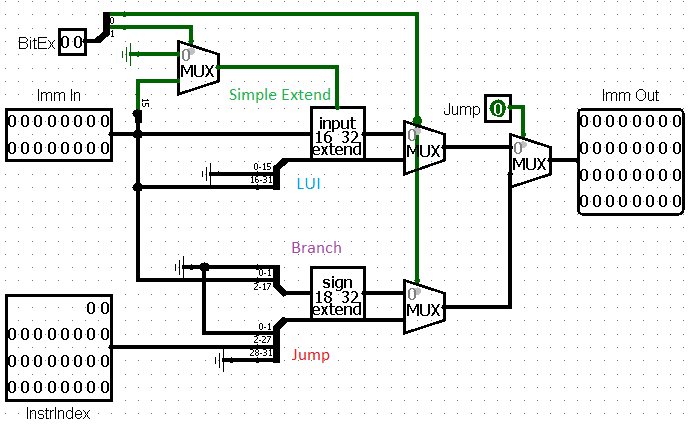
\includegraphics[width=0.6\textwidth]{BitExtend.png} \\
Figure 10: Bit Extender
\end{center}
\vspace{-1.4cm}
\end{wrapfigure}
Figure 10 shows the bit extender. This circuit will extend a portion of the instruction code into a 32-bit value that will be used in the Execute stage. \\
This circuit takes 4 inputs: \textbf{BitEx}, \textbf{Imm in}, \textbf{InstrIndex}, and \textbf{Jump}, and has 4 different types outputs:
\begin{enumerate}
\item
Simple Extend: This output is simply for 16-bit immediate values that must be bit extended. Bit 1 of BitEx determines whether we will sign extend or zero extend.

\item
LUI: This specific instruction has it's own extend method. The immediate value is instead extended on the right by zeroes.
\end{enumerate}

\begin{enumerate}
\setcounter{enumi}{2}
\item
Branch: Branching offsets are first extended on the right by 2 zeroes and then sign extended.

\item
Jump: Jumping is a bit different from the other outputs. Instead of a 16 bit immediate value, a 26 bit instruction index is used instead. 2 zeroes are extended on the right and 4 zeroes on the left.
\end{enumerate}

\subsubsection{Submodule D: Jump Disabler}

\begin{wrapfigure}{r}{0.4\textwidth}
\vspace{-1cm}
\begin{center}
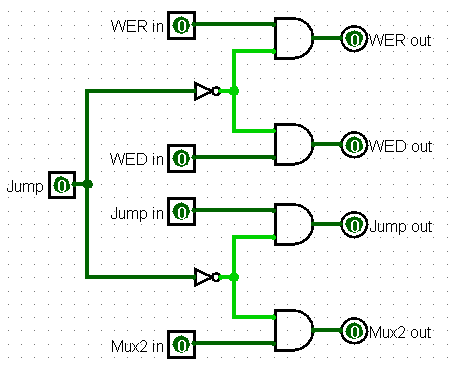
\includegraphics[width=.4\textwidth]{JumpDisable.png}\\
Figure 11: Jump Disabler
\end{center}
\vspace{-1cm}
\end{wrapfigure}
Figure 11 shows the jump disabler. \\
The purpose of this circuit is to clear an undesired instruction when jumps and branches are executed. This is necessary because our implementation of MIPS Pipeline is required to have only a single delay slot.\\
This jump disabler nullifies all functionality of an instruction by setting both write enables equal to 0, jump enable equal to 0, and the select bit of MUX 2 equal to 0. \\
We will later show that the value of MUX 2 is used for enabling load in the memory stage, which may cause stalling. By zeroing all 4 enables, we essentially disable the instruction from doing anything, although all computations will still be done.

\subsection{Correctness Constraints}
The functional requirements for this circuit are as follows:
\begin{itemize}
\item
The operation desired must be within this project's scope. The implemented instructions are: \textbf{ADDIU}, \textbf{ANDI}, \textbf{ORI}, \textbf{XORI}, \textbf{SLTI}, \textbf{SLTIU}, \textbf{ADDU}, \textbf{SUBU}, \textbf{AND}, \textbf{OR}, \textbf{XOR}, \textbf{NOR}, \textbf{SLT}, \textbf{SLTU}, \textbf{MOVN}, \textbf{MOVZ}, \textbf{SLL}, \textbf{SRL}, \textbf{SRA}, \textbf{SLLV}, \textbf{SRLV}, \textbf{SRAV}, \textbf{LUI}, \textbf{J}, \textbf{JR}, \textbf{JAL}, \textbf{JALR}, \textbf{BEQ}, \textbf{BNE}, \textbf{BLEZ}, \textbf{BGTZ}, \textbf{BLTZ}, \textbf{BGEZ}, \textbf{LW}, \textbf{LB}, \textbf{LBU}, \textbf{SW}, and \textbf{SB}.

\item
The values of Load Stall and Jump Enable must be correct in order for this stage to function correctly. As in the Fetch Stage, the program may get stuck if an incorrect value is given.
\end{itemize}

\subsection{Testing}
To verify the functional correctness of this module, we can simply input 32 bit instruction codes, and check if our outputs are as expected. However, there are far too many possible combinations of 32 bit codes to test. Thus, it is more optimal for us to check if each subcircuit is correctly implemented. \\

\noindent The subcircuit \textbf{Split} is trivial, as it does not involve any logic gates. \\

\noindent The subcircuit \textbf{Decode} can be checked by manually inputting each implemented function's \textbf{opcode} and/or \textbf{function code}, and seeing if the outputs are consistent with the ones on the table. \\ 

\noindent The subcircuit \textbf{Bit Extender} is trickier, because it deals with specific types of instructions. After checking that the Decode circuit is functioning properly, test programs with I and J type instructions should be ran to check the functionality of Bit Extender.

\noindent The subcircuit \textbf{Jump Disabler} is trivial, as it uses minimal gates. We can test it by running a test program with a jump instruction.

\section{Execute}
The Execute stage is where most of the computation of an instruction occurs.
\subsection{Circuit Diagram}
\begin{wrapfigure}{r}{0.26\textwidth}
\vspace{-3.8cm}
\begin{center}
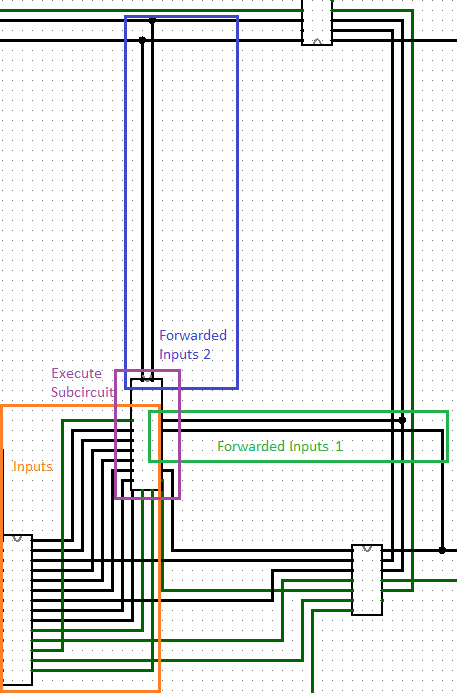
\includegraphics[width=.23\textwidth]{ALU.png} \\
Figure 12: Execute
\end{center}
\vspace{-.8cm}
\end{wrapfigure}
Our Execute stage is all condensed into a big Execute subcircuit, that does the computing, (with additional lower level circuits within the subcircuit) and a smaller subcircuit that aids in stalling. The Execute subcircuit gets its inputs mainly from the ID/EX registers but also from the EX/MEM and MEM/WB registers for use in the forwarding unit. The four outputs of the subcircuit is the main output C, the Write Enable for the Register File (which is conditional in the MOV instructions), a Jump variable, indicating whether or not we branch, and an output for Store functions. 

The Execute subcircuit has many subcircuits of its own. For each of the main inputs, A and B, with respective register addresses rs and rt, there is a forwarding unit that resolves data hazard issues that are present in this Mini-Mips processor. There is a multiplexor for B that chooses between B and the immediate. There are special sections that implement commands whose outputs do not come from the ALU. These commands include SLT, SLTI, SLTIU, and SLTU; MOVZ and MOVN; jumps and branches; and SW and SB. \vspace{-.2cm}
\begin{center}
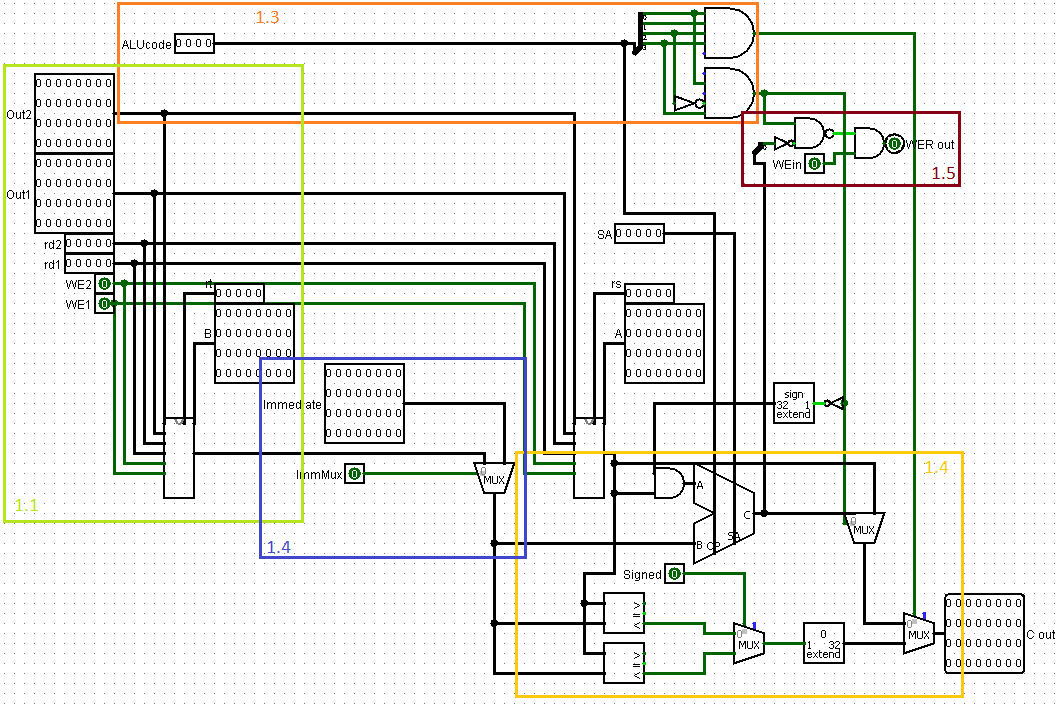
\includegraphics[width=14cm]{EXOVER.png}\\
Figure 13:Execute (Refer to this diagram for many of the subcomponents)
\end{center}

\subsubsection{General Purpose ALU}
The ALU (1.3) provides us the output for many of the simpler commands, and also provides us some intermediate outputs for the more specialized commands. Inputs A and B are determined by the specified command, but here we take them as given. We get the Op Code for the ALU as an input (1.1), and the SA is determined in a subcircuit (1.2), depending on whether or not the shift command was variable. 

\subsubsection{Forwarding Unit}
\begin{wrapfigure}{r}{0.27\textwidth}
\vspace{-1.5cm}
\begin{center}
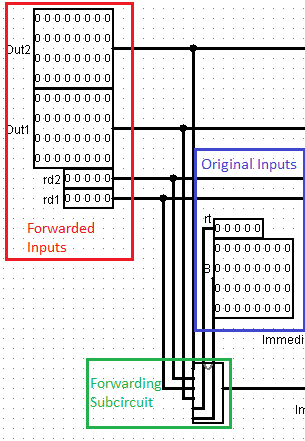
\includegraphics[width = 0.27\textwidth]{Forward1.png} \\
Figure 14: Forward
\end{center}
\vspace{-5cm}
\end{wrapfigure}
This part of the circuit compares the register address (rs) of a main input (Out0) with the write destinations of the instruction in the next stage (rd1) and the stage after that (rd2). Out1 and Out2 are to be written in those destinations respectively. The write enable bits from those stages need to be included as well. The Forwarding Unit takes these 8 inputs and chooses one of the 3 32-bit outputs Out0, Out1, Out2. Figure 14 shows the layout of the Forwarding Unit and its inputs in the Execute circuit.

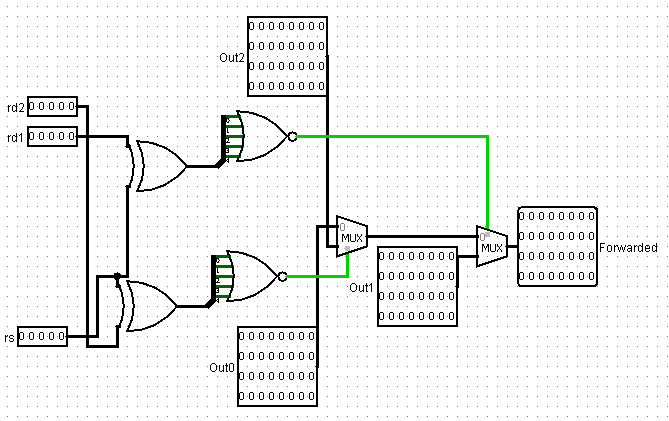
\includegraphics[width = 0.65\textwidth]{Forward2.png}

\hspace{1.5cm}Figure 15: Forward (subcircuit) \\

\noindent The Forwarding Unit compares the register addresses using an XOR and a NOR gate, to get a multiplexor selector, that is, if the register addresses are equal, we get 1, and otherwise 0. This is ANDed with a write enable bit. This is done for each rs and rd1, and rs and rd2. We first choose between Out0 and Out2 by comparing rs and rd2, then the selected and Out1 by comparing rs and rd1. This process automatically gives Out1 higher priority than Out2; if all of rs, rd1, and rd2 are equal, Out1 will be chosen over Out2. 

\subsubsection{Immediate MUX}
\begin{wrapfigure}{r}{0.3\textwidth}
\vspace{-1.8cm}
\begin{center}
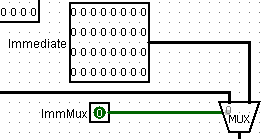
\includegraphics[width=.3\textwidth]{Immediate.png}\\
Figure 16: Immediate 1
\end{center}
\vspace{-1cm}
\end{wrapfigure}
This section (3.1) determines which of input B or the Immediate become an input for the ALU and the Comparators.\\
The upper MUX determines the second input of the ALU. The Immediate is already bit extended to 32 bits, and our Decoder gives us a multiplexor selector bit ImmMux that we use here. \\

\begin{wrapfigure}{l}{0.28\textwidth}
\vspace{-1cm}
\begin{center}
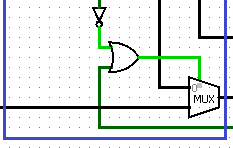
\includegraphics[width=.28\textwidth]{Immediate2.png} \\
Figure 17: Immediate 2
\end{center}
\vspace{-3cm}
\end{wrapfigure}
\noindent The lower MUX determines the second input of the Comparators. The difference between this MUX and the upper MUX is that the MUX will choose input B if the command is a Branch command, overriding the ImmMux. 

\newpage
\subsubsection{MOVN/MOVZ}
MOVN and MOVZ are one of the sets of commands that require special attention. The large AND gate in (4.1) outputs 1 if the ALU Op code is 1x01. Directly right of the AND gate is a subcomponent that disables the Register Write Enable if the ALU returns 0 for the comparison. \\
The AND gate in (4.3) replaces input A with a 32-bits of all 0's if the command is MOVN or MOVZ. This is because these commands' conditionals compare against zero. \\
Finally the output that is eventually stored if the conditional is true is the input A. Our MUX in (4.2) does exactly that, choosing input A over the ALU output C if the selector bit is 1.

\subsubsection{Comparator}
\begin{center}
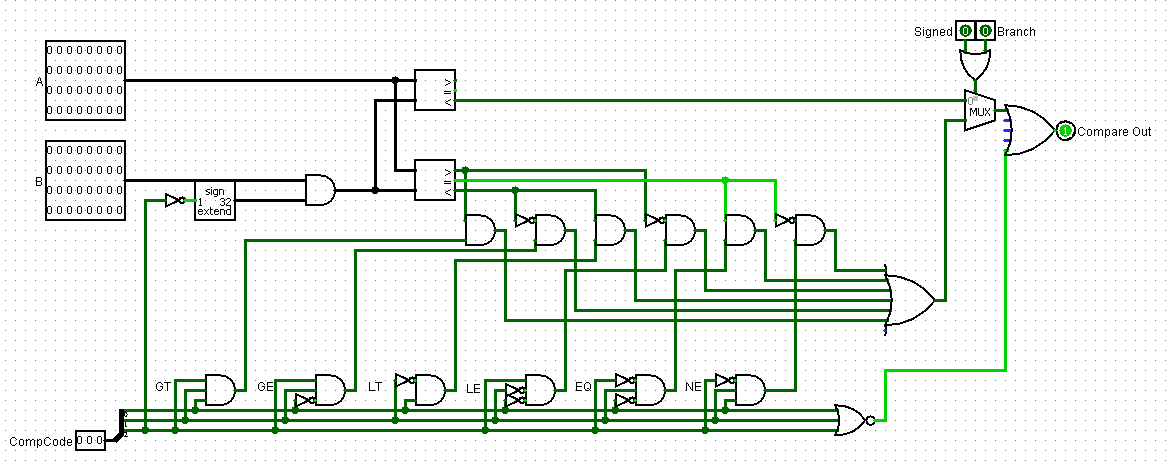
\includegraphics[width=.9\textwidth]{Compare.png}\\
Figure 18: Comparator
\end{center}
The Comparators (5.3) is used for the SLT commands and the branch commands. The upper comparator is unsigned and used for the commands SLTU and SLTIU. \\
We use a Comp Code that tells us the exact comparison that we want. \\
\begin{center}
\begin{tabular}{| c | c |}
\hline 
LEZ & 100 \\ \hline
LTZ & 101 \\ \hline
GEZ & 110 \\ \hline
GTZ & 111 \\ \hline
\end{tabular} \hspace{4cm}
\begin{tabular}{| c | c |}
\hline 
SLT & 001 \\ \hline
EQ &  010 \\ \hline
NE &  011 \\ \hline
\end{tabular}
\end{center}

\textbf{Design Decisions}
\begin{itemize}
\item
We set all the Comp Codes for comparisons with 0 to 1xx, so we sign extend the negation of the most significant bit of the Comp Code to control the second input to the comparators. 
\item
We represent GE and LE as the negation of LT and GT respectively and that can be seen in the first row of AND gates under the second comparator.
\item
Only 1 of the outputs from the second row of AND gates is 1 for any Comp Code. That means only 1 of the outputs from the first row of AND gates can be 1, and the big OR gate will output 0 unless that specified comparison is true. 
\item
The Comp Code for all other commands is 000, which makes the output of the subcircuit 1 regardless of the inputs. This is required so that Jump instructions always jump.(see (6.3))
\end{itemize}

Back in the Execute circuit, the Op code 1111 identifies the command as one of the SLT commands, and the MUX in (5.2) and the selector bit in (5.1) choose the zero extended Comparator output to be the final output. 

\newpage
\subsubsection{Jump and Branch}
Jumps and Branches also require special computing. \\
\begin{wrapfigure}{r}{.6\textwidth}
\vspace{-1cm}
\begin{center}
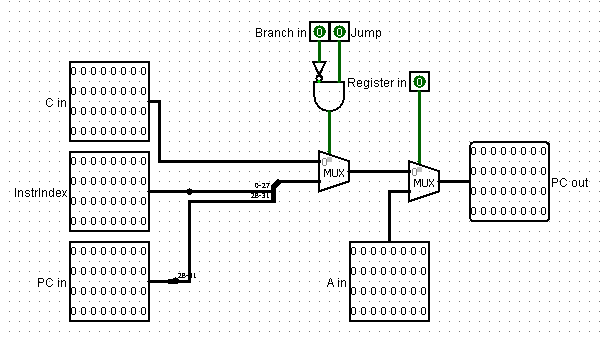
\includegraphics[width=.6\textwidth]{Jump.png}\\
Figure 19: Jump and Branch
\end{center}
\vspace{-1cm}
\end{wrapfigure}
The branch conditionals are done in the Comparator (see above) which then turns off or maintains the Jump variable in (6.3). The target address for a branch is computed in the ALU. The PC in (6.1) is incremented by 4 and then chosen for in the MUX in (6.2) to be the first input of the ALU. \\
The target address for a jump is computed in a separate subcircuit, which is done simply by using splitters. \\
The subcircuit also chooses between the jump target address and the branch target address and address stored in a register depending on the related bits. 

\subsubsection{Store Output}
In (7.1), we simply output the input B which is stored in RAM in the instructions SW and SB.

\subsubsection{LoadStall Disable}
This small subcircuit in the main circuit simply disable the Jump variable, Load Enable, Register File Write Enable, and RAM Write Enable in the Execute stage during a stall. These 4 variables when all disabled effectively prevent the instruction from doing anything.

\subsection{Correctness Constraints}
\begin{itemize}
\item The correctness of this module depends on the correctness of the inputs that are decoded in the Instruction Decode stage. Therefore, one functional requirement is that the inputs are consistent with the MIPS command given. For instance, WE in (write enable) must be 1 if the command ultimately writes back to the Register File. 
\item The module takes inputs from the Memory and Write Back Stages. Therefore, these stages need to be implemented correctly in order for this stage to be correct.
\item The execute subcircuit in this implementation is only correct for the instructions in Table A and Table B. Only these instructions can be given in the Instruction Fetch Stage.
\item There are also certain limitations on the ordering of instructions given, namely that a Jump or Branch cannot be given in the delay slot of another Jump or Branch. However this is a limitation on the whole circuit, not on the Execute stage itself.

\end{itemize}

\subsection{Testing}
A large portion of the instructions depend on the correctness of the ALU circuit. Since that is given to us, we assume its correctness. For those instructions, computation is given correct, so we only have to test one case for each, that is, if one case gives us the correct nontrivial output (like 0 or something that could have been an accident), then the data path was correct and all inputs for that instruction should give us a correct output.  \vspace{-.2cm} \\

\noindent For the function that are not computed solely using the ALU, we need to check an encompassing set of cases. Many of the Table B instructions' correctnesses are not solely dependent on the execute stage, but the overall testing for those instructions will be mentioned here. Load and Store will be elaborated more in Memory.  \vspace{-.2cm} \\

\noindent For the SLT, MOV, and Branch instructions, we check all the cases for the conditionals, namely less than, greater than, and equal. For branches we need to check if the delay slot works properly and if the instruction after the delay slot is canceled properly. We also check if branching with both negative and positive offsets work properly. \vspace{-.2cm} \\

\noindent For the Jump instructions, we check if the delay slot works properly and if the instruction after the delay slot is canceled properly, as in the Branch tests. The register Jumps also need to be tested, and we have to check if the link address is stored properly in JAL and JRAL. \vspace{-.2cm} \\

\noindent Load and Store only have their addresses computed in the ALU in the Execute stage, which is trivial. The bulk of their correctness is dependent on the Memory stage. \vspace{-.2cm} \\

\noindent Lastly, we need to test the forwarding unit. We need to test for EX/MEM $\rightarrow$ EX forwarding and MEM/WB $\rightarrow$ EX forwarding. We test with multiple cases to be safe.  \vspace{-.2cm} \\

\section{Memory}
The Memory stage is where data is stored.
\subsection{Circuit Diagram}
\begin{wrapfigure}{r}{.4\textwidth}
\vspace{-3cm}
\begin{center}
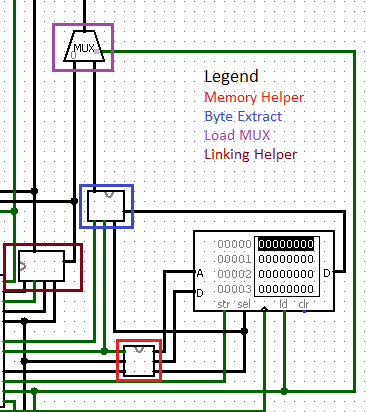
\includegraphics[width=.4\textwidth]{MemOver.png} \\
Figure 20: Memory
\end{center}
\vspace{-2.5cm}
\end{wrapfigure}

Our Memory stage has 3 main subcircuits:
\begin{enumerate}
\item
The Memory Helper processes the outputs from the Execute stage to give us the Byte Selector, the 20 bit Memory Address, and the RAM input. 

\item
The Byte Extract, much as the name suggests, extracts the byte from RAM output in LB and LBU instructions, and does nothing otherwise.

\item
The Linking Helper processes outputs from the Execute stage to set rd to 31 and choose the address to be written.
\end{enumerate} 
There is also a MUX that chooses for the RAM output if the Load Enable is on.
 
\subsubsection{Memory Helper}
\begin{wrapfigure}{r}{.6\textwidth}
\vspace{-1.4cm}
\begin{center}
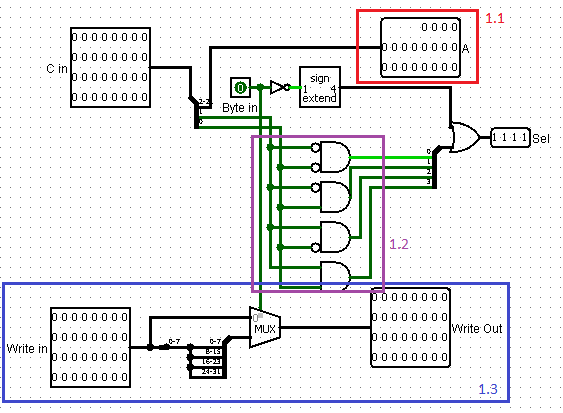
\includegraphics[width=.6\textwidth]{MemHelp.png}\\
Figure 21: Memory Helper 
\end{center}
\vspace{-.5cm}
\end{wrapfigure}
The first output in the Memory Helper is the Write Address A (1.1). This is acquired by simply extracting bits 2-21 from the main Execute output C. \\
The second output is the RAM input (1.3). This is either the original Write in if the instruction is SW or its first byte replicated 4 times if the instruction is SB. ("Byte in" indicated whether the memory instruction is Word(0) or Byte (1)) \\
The final output is the Byte Select. The AND gates in (1.2) extract from the first 2 bits of "C in" the Byte information. Only one of the AND gates can output 1 at a time, so our Byte Select is for the most part limited to one of 0001, 0010, 0100, and 1000, which is what we want. The exception to this rule is when the instruction isn't a Byte instruction, in which case the Byte Select is 1111, which we get by using an OR gate with the negation of "Byte in", sign extended. 

\subsubsection{Byte Extract}
\begin{center}
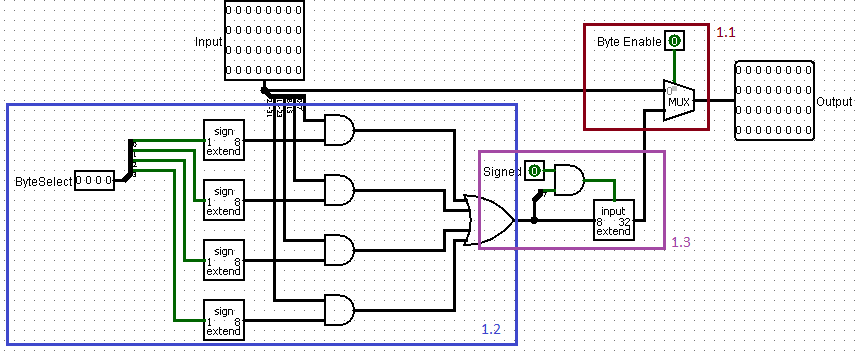
\includegraphics[width=.9\textwidth]{ByteExtract.png} \\
Figure 22: Byte Extract
\end{center}
 The Byte Extract, much as the name suggests, extracts the byte from RAM output in LB and LBU instructions, and does nothing otherwise.\\
 From the MUX in (1.1), the output is just the original input if the memory instruction is a word instruction. \\ 
 In (1.2), since the Byte select will only have 1 nonzero bit if the memory instruction is a byte instruction, 3 of the sign extends will output all 0s and 1 will output all 1s. Each of them are ANDed with a byte from the Input; only one of those bytes will retain its information. These 4 lines are ORed and we are left with the byte that we need to extract. Finally in (1.3), the byte is zero extended or sign extended according to the instruction.
 
\subsubsection{Linking Helper}
\begin{wrapfigure}{r}{.4\textwidth}
\vspace{-1cm}
\begin{center}
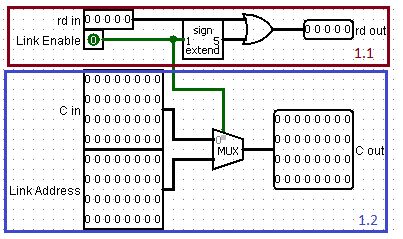
\includegraphics[width=.4\textwidth]{Linking.png}\\
Figure 23: Linking Helper
\end{center}
\vspace{-2cm}
\end{wrapfigure}
This subcircuit is relatively simple and only exists to simplify the main circuit. In (1.1), "rd out" is either the original "rd in", or 31 if we are linking. The 31 is created by sign extending the linking variable to 11111.\\
"C out", the word that we want to store in rd, is simply chosen for by a MUX.

\vspace{1cm}

\subsection{Load Stall and Jumping}
\begin{center}
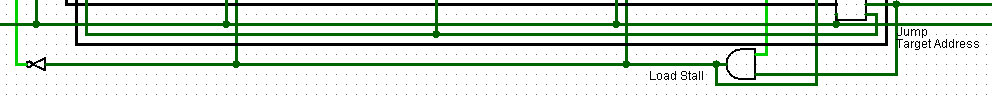
\includegraphics[width=.9\textwidth]{Disable.png} \\
Figure 24: Disable
\end{center}
Load Stalling and Jumping happen when the instruction reaches the Memory Stage. The Load Stall line is achieved by ANDing the Load Enable and the output from the Execute Stage indicating whether or not the rs and rt from the Execute Stage coincide with the rd in the Memory Stage. The Jump Variable is just given from the EX/MEM registers. \\
Our Load Stall works by disabling the IF/ID, ID/EX, and PC registers and disabling the Jump Variable, Load Enable, and the two Write Enables in the Execute Stage (effectively canceling the instruction). \\
Our Jump also disables the same 4 variables, but in the Decode Stage, which is the instruction after the Delay Slot. The target address and the Jump Variable are fed into the Instruction Fetch Stage to do the actual Jump.

\subsection{Correctness Constraints}
\begin{itemize}
\item
Assuming all preceding stages are correct, the main constraint for the Memory Stage is the RAM Write Address has to be a valid word address if the associated memory instruction is a word instruction. Technically our circuit would treat the address as if the first two bits indicating bytes were 0s. We don't have a method to call an error, thus we are limited in this way.
\item
Another constraint arises from the fact that our RAM only supports 20 bit word addresses, so the base + offset in our memory instructions can be at most 22 bits long. Practically, the other 10 bits don't have to be 0s, but the range that the ROM sets RAM addresses must be within 22 bits. For this project, we assume that RAM addresses are between 00000000 and 000fffff. 
\end{itemize}

\subsection{Testing}
Testing for the Memory Stage is essentially testing memory instructions.\\\vspace{-.2cm}

\noindent 
Load Word is tested by storing a word first, then loading it into the register file, so it makes sense to test Store Word first.\\\vspace{-.2cm}

\noindent 
Testing Store Word is basically checking if the word is stored, and if it is stored in the right address. Similarly Store Byte is tested by checking if the least significant byte is stored in the right byte address. We test the byte addressing for each possible Byte Select (0001, 0010, 0100, 1000). The memory address calculation is assumed to be correct from the Execute Stage. \\\vspace{-.2cm}

\noindent 
Additionally we test Store Word with multiple forwarding instances.\\\vspace{-.2cm}

\noindent 
For Load Word when we check if the correct value is loaded, the word just has to match the word in the RAM. Load Byte we also want to make sure that the correct byte is extracted and that it is in the least significant bits, and that it is sign extended correctly. Load Byte Unsigned is the same as Load Byte except we need to make sure that it is always zero extended.\\\vspace{-.2cm}

\noindent 
Other than the main output, we need to check whether or not the Stall works properly. We make sure that 1 step forwarding stalls properly. We also make sure that 2 step forwarding does not stall and that non forwarded Load instructions don't stall. \\ \vspace{-.2cm}

\noindent Jumping is mentioned above in the Execute Stage Testing.

\section{Writeback}
The Writeback Stage only has one core functionality which is to store a value in a register if the write enable is 1. The only piece of circuit that isn't wiring in this Stage is the given Register File, so as long as our inputs are correct, there is no need to test this stage.

\section{Summary}
The design of \textbf{Project 2: Fully Pipelined MIPS} consisted of adding to the Decode and Execute stages and implementing the Memory stage, in which jumping, branching, storing, and loading occur.  \\

\noindent In order to implement all of the operations required, we have to differentiate each one. We do this by creating extra variables to pass through decode (in addition to the universally required variables such as \textbf{Write Enable}). For instance, because we have both signed comparison as well as unsigned comparison, the value \textbf{Signed} was created to differentiate the two. That value is passed into the Execute stage, which is then used as the select bit of a multiplexor. An example of a value required for Project 2 is the value \textbf{Branch}. It is important to differentiate branching and jumping, since branching requires a condition to be true. Branch was created for that reason.\\

\noindent After having all of the information required the instruction is executed in the Execute stage. Since functionality of the the supplied ALU does not cover all, we have to add more pieces to our Execute stage. These pieces include a forwarding unit, immediate multiplexors, a universal comparator, and a special jump and branch address calculating circuit. \\

\noindent The Memory stage, newly introduced in Project 2, allows us to store significantly more data. It required only a few small subcircuits in addition to the provided MIPS RAM. The implementation of linking is done here, as well as the differentiation between Byte and Word memory operations. Furthermore, all values related to jump are sent to the rest of the CPU during this stage.  \\

\noindent While the pipeline is much more advanced in Project 2 than in Project 1, the Instruction Fetch and Writeback stages are still fairly simple. For Project 2, a small subcircuit is added for the implementation of jumps and branches, however the latter is exactly identical to how it was previously. \\

\noindent With the addition of Memory and Jumps, it is now possible to implement much more complex programs that require recursion and/or large amounts of data.
\end{document}